\documentclass[11pt,a4paper,oneside]{article}
\usepackage[usenames,dvipsnames,svgnames,table]{xcolor}
\usepackage[utf8]{inputenc}
\usepackage[T1]{fontenc}
\usepackage[english]{babel}

% Next two line are two change the font being used
\usepackage[scale=0.8]{tgheros}
\renewcommand{\familydefault}{\sfdefault}

\usepackage{graphicx}
\usepackage{subcaption}
\usepackage{float} % Para poder usar headers nas imagens
\usepackage{geometry}
\usepackage{amsmath} % Para usar comandos de matriz
\usepackage{mathtools} % Para usar texto nas sextas nas equations
\usepackage{wrapfig}  %
\usepackage{hyperref} % To use urls
\usepackage{multicol} % To use columns on some parts of the guide
\setlength{\columnsep}{0.75cm}

\geometry{a4paper, top=1.5cm, bottom=2.5cm, left=1.60cm, right=1.60cm, marginpar=0cm}
\setlength{\parskip}{0.5em}
\renewcommand{\baselinestretch}{1.1}

\setcounter{section}{1}

\title{\textbf{Artificial Intelligence and Decision Systems \\ Mini-Project I}}
\author{Pedro Ferreira - 75263 \hspace{1.5cm} Rúben Tadeia - 75268}
\date{Group 14}

\begin{document}

\maketitle

\vspace{-14mm}

\setcounter{section}{0}

\section{Formulation of the problem}

This mini-project addresses the problem of scheduling the launch of components to assembly a large structure in orbit, given a set of components to be launched, a construction plan and a list of launches with certain specifications. The goal is to do so minimizing the total cost. In order to solve the problem there will be a clear distinction between the components already in space, the components still in Earth and the launches that have already been used. To characterize this it is sufficient to have the problem state representing the set of actions already used until that moment. Therefore the \textbf{problem state} will be a list with a tuple for each action, being each tuple composed of a string with the launch ID, a set (python structure) with the components sent of that specific launch and the cost of that action. The representation will look like this $[ (date_1, {components_1}, cost_1), ..., (date_n, {components_n}, cost_n) ]$. In terms of \textbf{operator}, the possible actions for a given actual state will be obtained by a series of logical steps, further explained in figure \ref{fig:possible_actions}. Some extra cautions were taken, such as having the list of launches ordered by maximum payload, so that, when a given combination of components doesn't "fit" in one launch, it won't fit in any of the others. The \textbf{initial state} is defined to be an empty list, since there are no components in space initially, as defined in the project description \textit{"Note that initially there is no component in orbit"}. The \textbf{goal state} will be defined as the state in which the union of the sets with components for all its taken actions has all the components that needed to be sent to orbit. Finally, the \textbf{path cost} will be defined as the sum of the cost of all the actions taken to achieve a given state.

\begin{figure}[H]
    \centering
    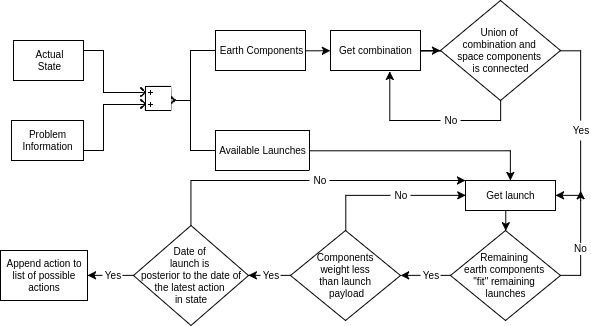
\includegraphics[width=10cm]{images/new_possible_actions.png}
    \caption{Simplified sequence of steps in order to get a list of possible actions for a given actual state}
    \label{fig:possible_actions}
\end{figure}

\section{Search algorithms implemented}

\textbf{Uninformed search:} In terms of uninformed search, the chosen algorithm was the \textbf{uniform cost search}. In the conditions of this problem, with positive step costs, \textit{g(n)}, it is guaranteed that the behaviour of the algorithm is both complete and optimal, meaning that the solution it returns is the optimal one. The complexity of this algorithm is $O(b^{1 + C^{*}/\epsilon})$ for both space and time.

\hspace{-6mm}\textbf{Informed search:} 
Given that the uninformed search may take more time and space than one has available, informed search is often a valuable alternative. The key difference between this and uninformed search is the utilization of a \textbf{evaluation function}, \textit{f(n) = g(n) + h(n)}, meaning that besides the path cost, \textit{g(n)}, a heuristic function \textit{h(n)} is also used. The informed search method used was the \textbf{A*}. The complexity of this algorithm is $O(b^d)$ for both time and space, being its advantage the fact that, by making use of a heuristic function, it will expand less nodes than its uninformed counterpart. For a tree-search, like the problem that is being tackled, the A* is optimal and complete if the heuristic function is \textbf{admissible}, meaning that the heuristic \textit{h(n)} never overestimates the true cost to the goal. 

\section{Heuristic function developed}

In order to get the optimal solution using the A* algorithm, an admissible heuristic was developed, which means, as previously said, that the heuristic $h(n)$ should never overestimate the true cost of the goal, $h(n) \leq h^*(n)$. Another way to prove that an heuristic is admissible is to prove that it is \textbf{consistent}, meaning that the heuristic satisfies the triangular inequality, $h(n) \leq c(n, a, n') + h(n')$, since consistency implies admissibility. It's also worth noting that the value of the heuristic function for the goal state has to be zero.

\hspace{-6mm}The developed heuristic is a function of the actual state that returns the total weight of the components still on Earth times a variable cost, \textit{v}. The reasoning behind this is that we want to have the minimum value in components on Earth as soon as possible. This variable cost was defined in a way to make the heuristic consistent and therefore, admissible. Being $F_i$ and $V_i$ the fixed cost and variable cost of a launch, $W_i$ the sum of the weight of the transported components of a given action, and $W^A$ and $W^B$ the weights of the components on Earth after and before the action and since all these variables are greater or equal than zero, for the resulting inequality of equation \ref{eq:1} to be true, \textit{v} has to be smaller or equal to $V_i$. Since there are several launches, \textit{v} has to be smaller than the lowest variable cost of the available launches. It's worth noting that $W^A - W^B = W_i$. This way it is proved that the proposed heuristic is consistent, admissible and therefore allows to obtain an optimal solution using A* algorithm.

\vspace{-3mm}
\begin{equation}
    h(n) \leq c(n, a, n') + h(n') \Leftrightarrow W^B \textit{v} \leq F_i + V_i W_i + W^A \textit{v} \Leftrightarrow 0 \leq F_i + V_i W_i + (W^A - W^B) \textit{v} = F_i + W_i (V_i - \textit{v})
\label{eq:1}
\end{equation}

\section{Performance of the heuristic functions}

In order to test the performance of our heuristic function, the results from the uninformed and the informed search were compared, with respect to the key metric for this kind of evaluations, the \textbf{effective branching factor}, obtained by solving $N = b^* + (b^*)^2 +...+ (b^*)^d$ with respect to $b^*$. These results may be seen in table \ref{table:1}.


\begin{table}[H]
\centering
\caption{Results of both Search's for different files}
\label{table:1}
\begin{tabular}{ccccc}
 & \multicolumn{2}{c}{\large\textbf{Uniformed  Search}} & \multicolumn{2}{c}{\large\textbf{Informed  Search}} \\
\textbf{Filename} & \textbf{Nodes Expanded} & \textbf{Branching Factor} & \textbf{Nodes Expanded} & \textbf{Branching Factor} \\
trivial1.txt & 11 & 1.74 & 11 & 1.74 \\
trivial2.txt & 18 & 17.00 & 11 & 10.00 \\
simple1.txt & 566 & 3.31 & 566 & 3.31 \\
mir.txt & 40842 & 34.17 & 32071 & 31.43 \\
pers1.txt & 11 & 1.74 & 11 & 1.74 \\
pers2.txt & 1411 & 2.31 & 1411 & 2.31 \\
pers3.txt & 7711 & 19.41 & 4479 & 16.14 \\
pers4.txt & 163 & 5.08 & 158 & 5.02 \\
pers5.txt & 21 & 4.00 & 21 & 4.00
\end{tabular}
\end{table}

As it may be seen, the number of nodes expanded is always equal or less in the case of the informed search comparing to the uninformed search, as expected. It's worth noting that the reduction of expanded nodes is still below what one would expect from using an heuristic and that the branching factor is still very high in some cases. Nonetheless the benefit in terms of time consumed was noticeable for the larger problems, which shows the usefulness of using informed methods when performance is at stake.

\end{document}